\documentclass{article}

\usepackage[utf8]{inputenc}
\usepackage[margin=1in]{geometry}
\usepackage{graphicx}
\usepackage{amsmath}
\usepackage{amssymb}



\setlength{\parindent}{0pt}

\title{CMSC426 Project 3}
\author{Pavan Ravindra, Sabrina Zhou, Gaurav Guglani}
\date{Using 5 Late Days}

\def\Plus{\texttt{+}}
\begin{document}
	
	
	\maketitle
	
	For implementing rotobrush, we followed the systems diagram that was given to us:
	
	\begin{center}
		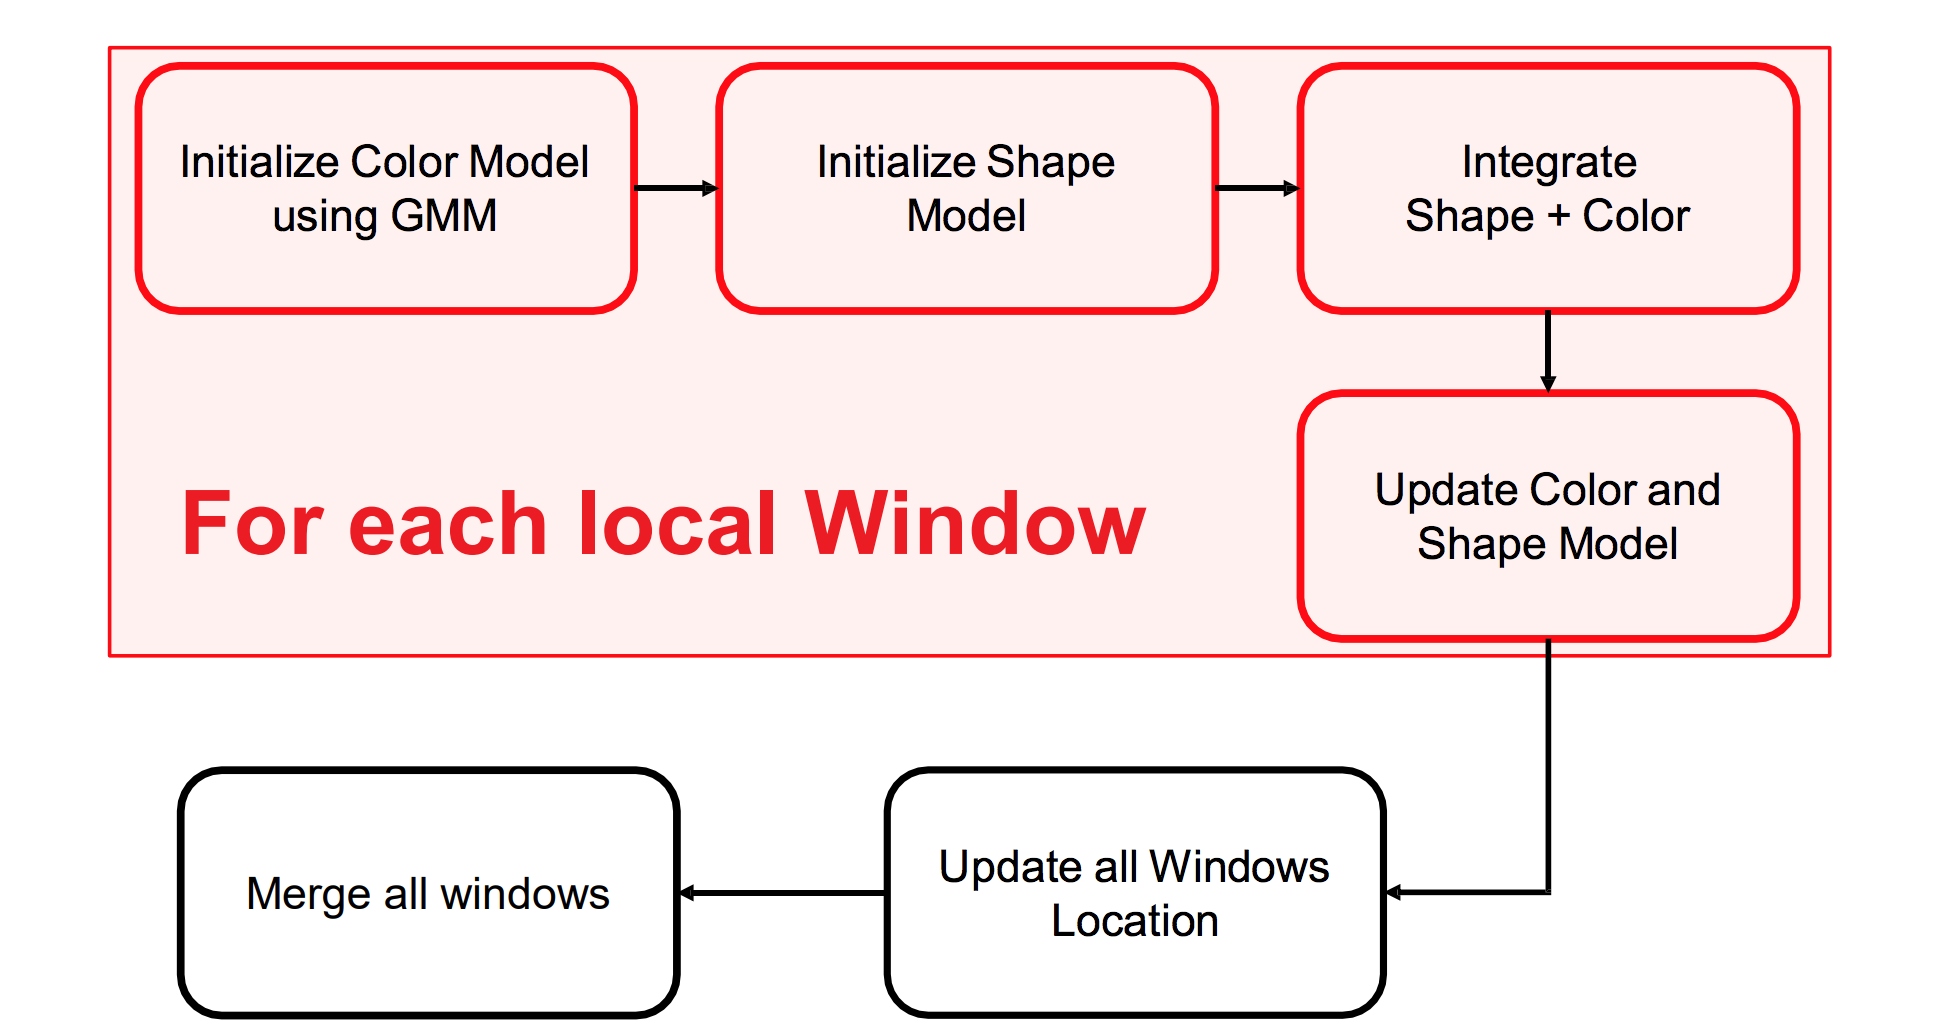
\includegraphics[width=104mm]{img/i1}
	\end{center}
	
	\section{Set Up Local Windows}
	To initialize the shape/color models, we needed to create local windows along the outline of each figure. Luckily, we were given initLocalWindows.m so all we had to do was use roipoly to make the mask. We chose to have 35 windows with a width of 45 pixels because we learned that we wanted to have as many points as possible without slowing the runtime. Below is an image with the local windows we had for the turtle. We initially had a width of 30 pixels because we wanted about 1/3 of the window to overlap with another, but our color models performed better when we increased it to 45. We also initially had 40 windows, but that took too long to run. 
	
	\begin{center}
		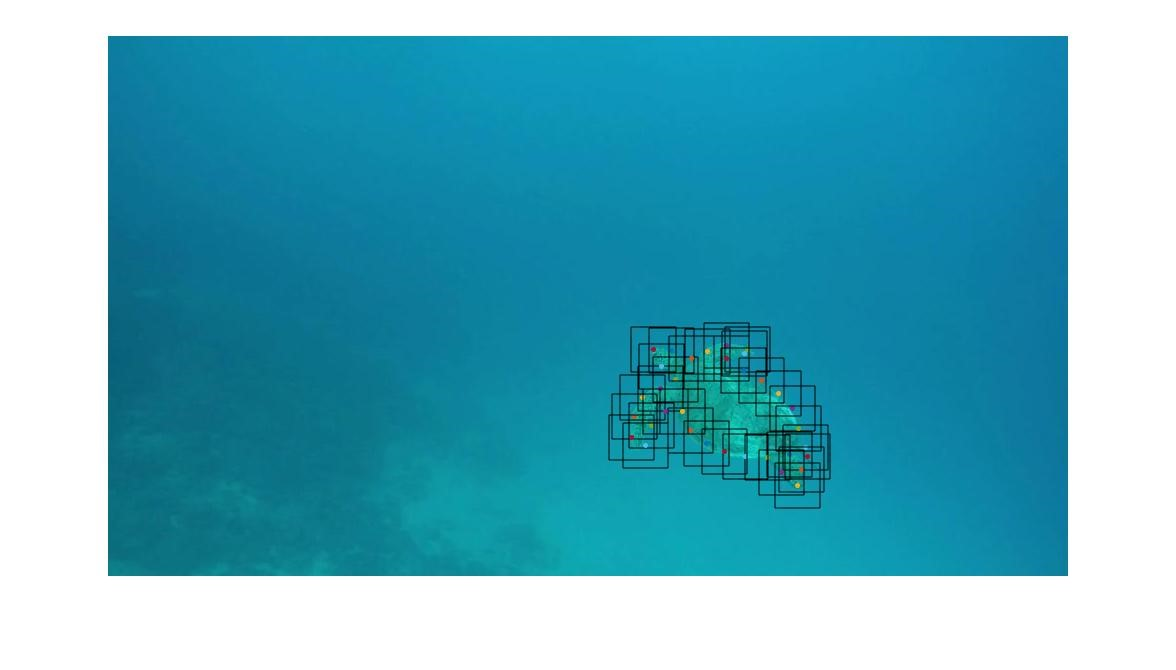
\includegraphics[width=104mm]{img/i2}
	\end{center}

	\section{Initialize Color Models}
	Creating the color models wasn’t too difficult in terms of the math, but figuring out what we wanted to store in color models was difficult. We decided to store for each window in a cell: color model confidence, GMM for background and foreground, local windows, the points in the foreground and background, distance from points to the mask, and foreground probability for each point. We initially only had confidence, GMM, distance, and probability. We, then later added local windows, and points when we wrote the updateModels file because we realized that we still needed those. For the math, we followed what was in the slides to calculate foreground probability and confidence.
	Here is an image of a window on the left and what we calculated as the foreground probability on the right for a local window of the turtle:
	
	\begin{center}
		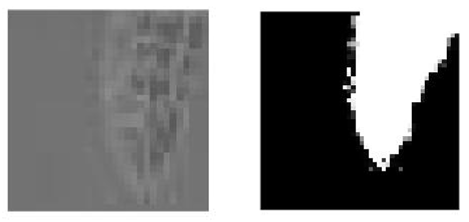
\includegraphics[width=100mm]{img/i3}
	\end{center}

	It’s a little off, but still retains the main shape.
	
	\section{Compute Color Model Confidence}
	
	To calculate color model confidence, we used: $$f_c = 1 - \frac{\int_{W_k}^{}|L^t(x)-p_c(x)|*\omega_c(x)dx}{\int_{W_k}^{}\omega_c(x)dx}$$. We used bwdist to calculate distance for $\omega$. To find $p_c$, we used $p_c (x)= \frac{p_c (x | F)}{(p_c (x | F)+p_c (x | B)}$ and the GMM and pdf to find the foreground probability. As you can see from the above images, we thought we did well with the results of the color model. Below is an image of the color confidence.
	
	\begin{center}
		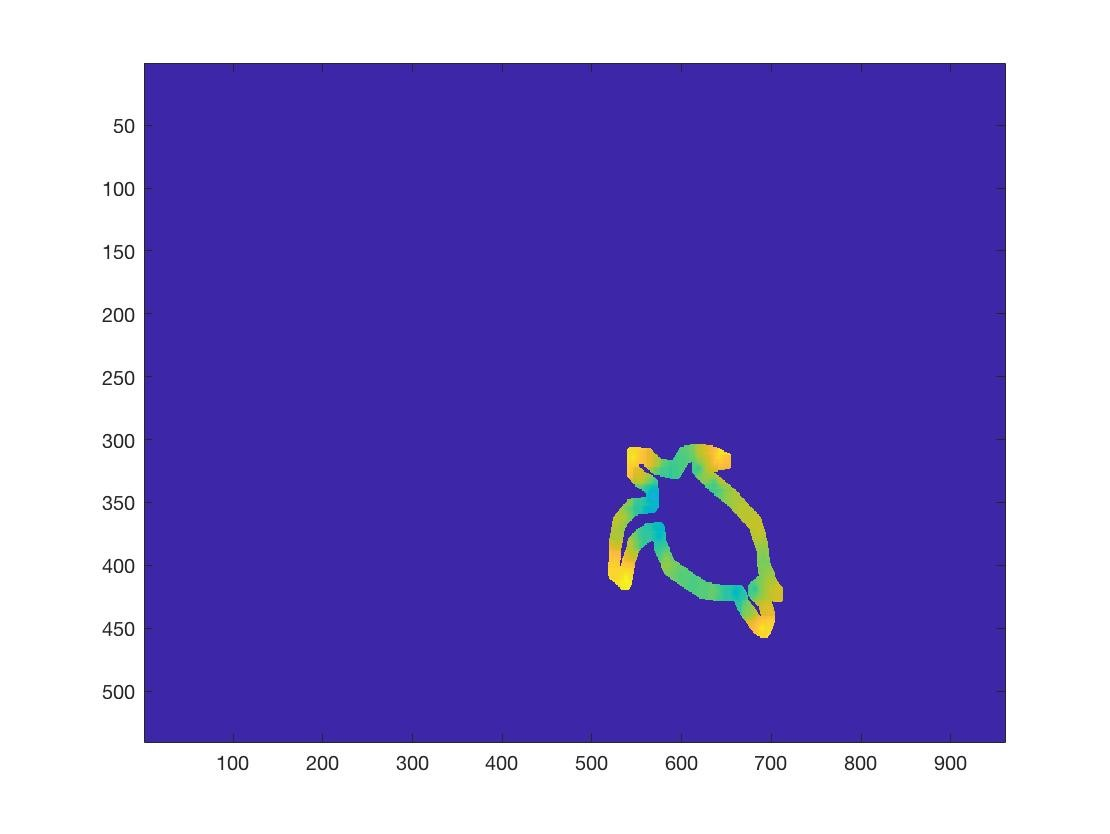
\includegraphics[width=100mm]{img/i4}
	\end{center}

	\section{Initialize Shape Model}
	Creating the shape models also wasn’t that difficult. The only thing we decided to store in it was the shape confidences. 
	
	\section{Compute Shape Confidence}
	
	To calculate confidence, we used the formula that was given to us:
	
	$$f_s(x)=1-exp(-\frac{d^2(x)}{\sigma^2_s})$$
	
	If $f_c$ was between $f_{cutoff}$ and 1, then $\sigma_s=\sigma_{min}+a(f_c-f_{cutoff})^r$. Otherwise, if it was between 0 and $f_{cutoff}$, then $\sigma_s=\sigma_{min}$. For the parameters, we used 0.85 for $f_{cutoff}$, 2 for R, and about 1700 for A. We got these numbers from the paper and a little bit of fine turning. Here is an example of a shape confidence we calculated:
	
	\begin{center}
		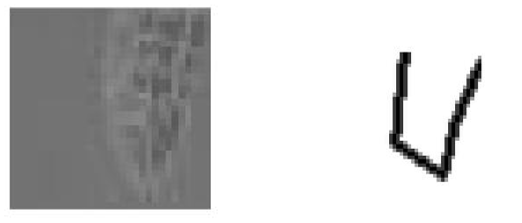
\includegraphics[width=100mm]{img/i12}
	\end{center}
	
	It looks a little off, but that may be because the parameters could’ve been adjusted a little better.
	
	
	\section{Estimate Entire Object Motion}
	For calculateGlobalAffine, we initially were using detectHarrisFeatures to get the features, but we weren’t satisfied with those results, so we switched to detectSURFFeatures. Below is a picture of the matched features on the first frame with the second frame after we extracted the features. 
	
	\begin{center}
		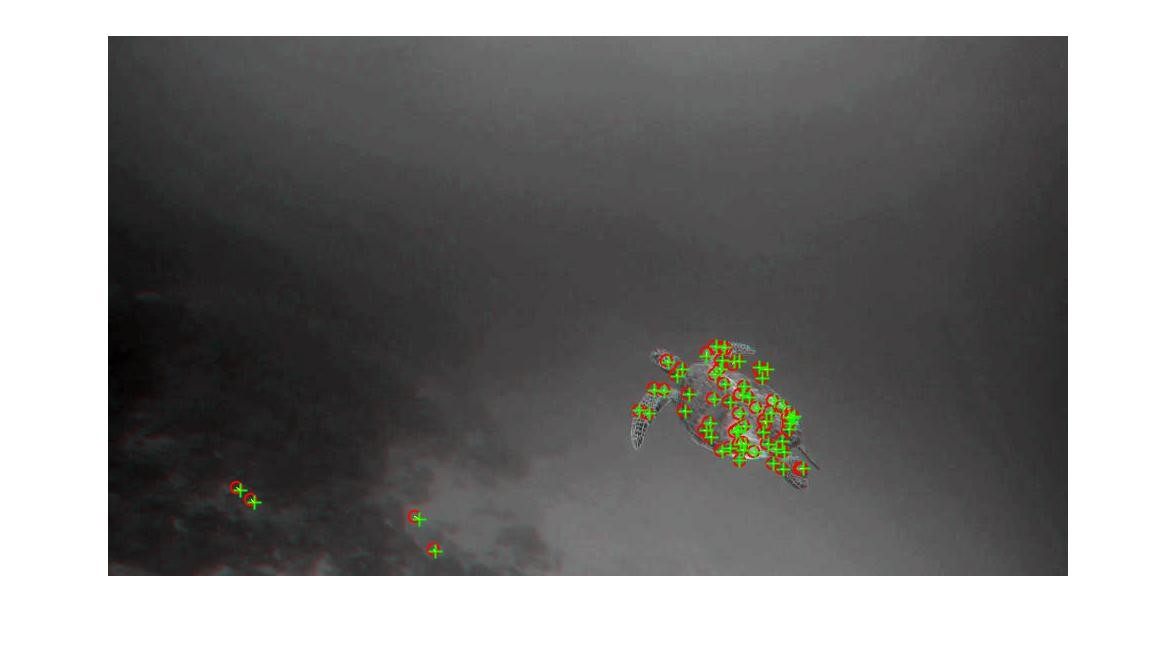
\includegraphics[width=100mm]{img/i5}
	\end{center}

	As you can see, there were some features that shouldn’t have been there on the left. We then filtered those out by checking if it was in the mask. The image below is what we got after this filtering. 
	
	\begin{center}
		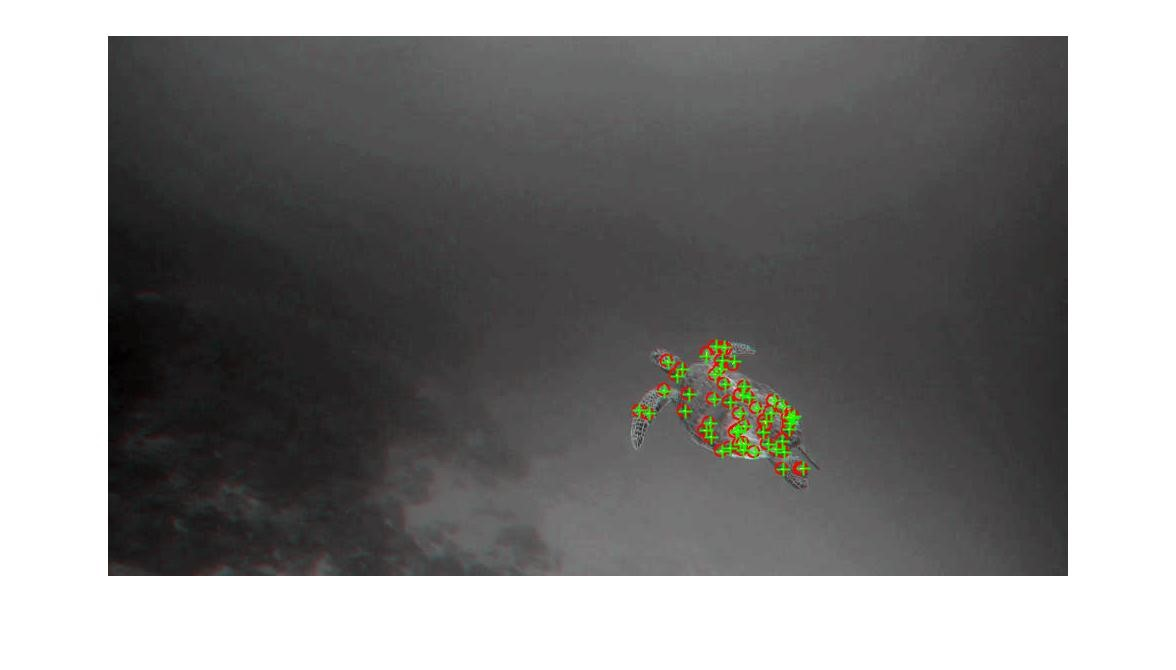
\includegraphics[width=100mm]{img/i6}
	\end{center}

	We then used estimateGeometricTransform, imwarp, transformPointsForward to get the warped mask, warped mask outline, warped frame, and new local windows.
	Below are images of the warped frame and warped mask, respectively.
	
	\begin{center}
		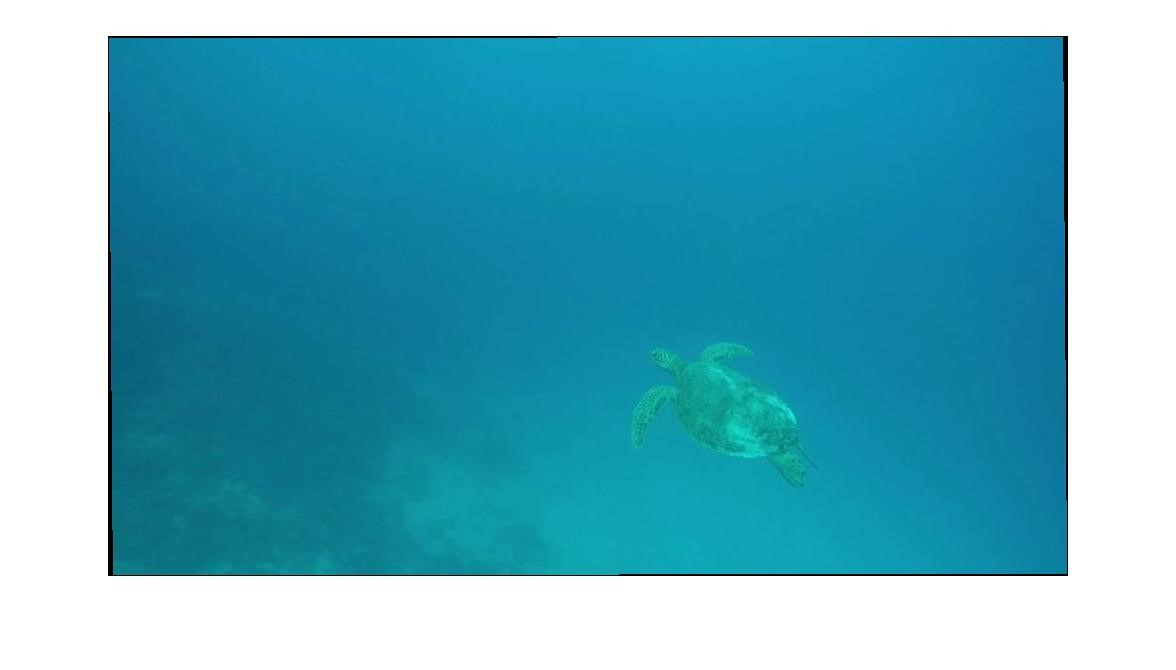
\includegraphics[width=100mm]{img/i7}
	\end{center}

	\begin{center}
		
\includegraphics[width=100mm]{img/i8}
	\end{center}

	\section{Estimate Local Boundary Deformation}
	For localFlowWarp, we used estimateFlow and opticalFlowFarneback. Below is an image of the optical flow object.
	
	\begin{center}
		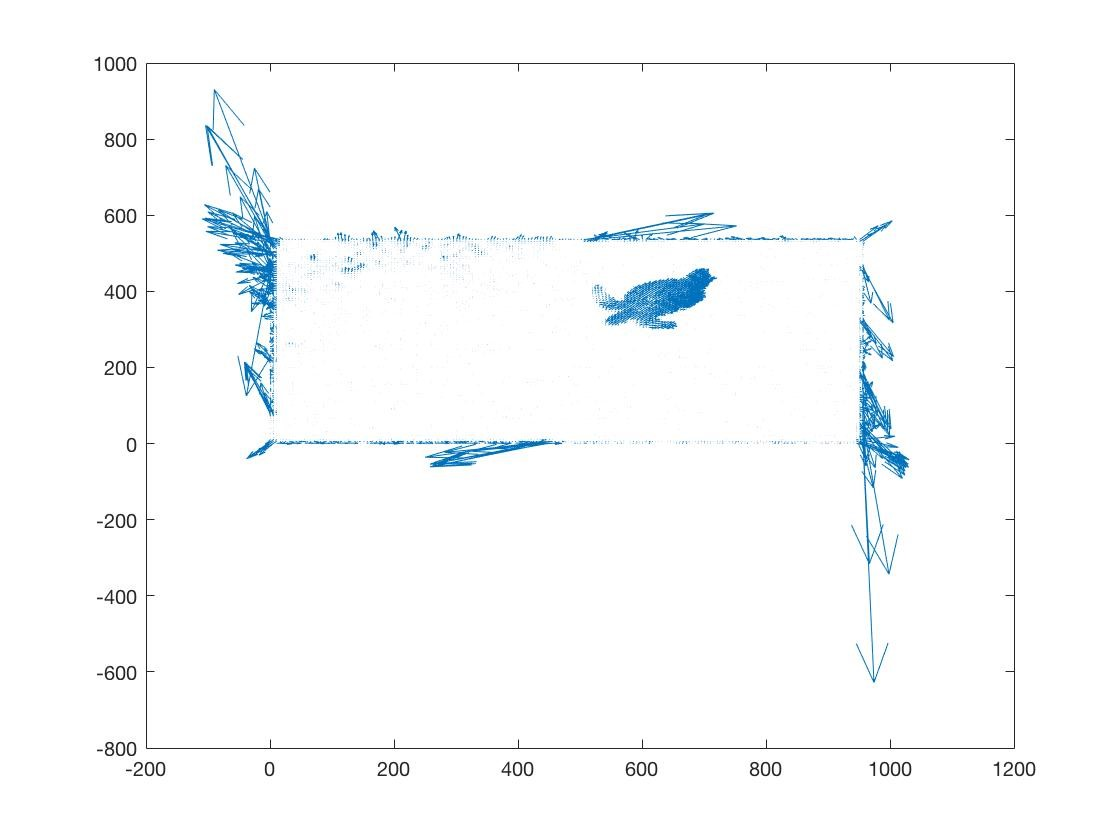
\includegraphics[width=100mm]{img/i9}
	\end{center}
	
	Then, we used $V_x$ and $V_y$ to get the new local windows from the old ones. We didn’t have any problems with this. Below is an image of the new windows.
	
	\begin{center}
		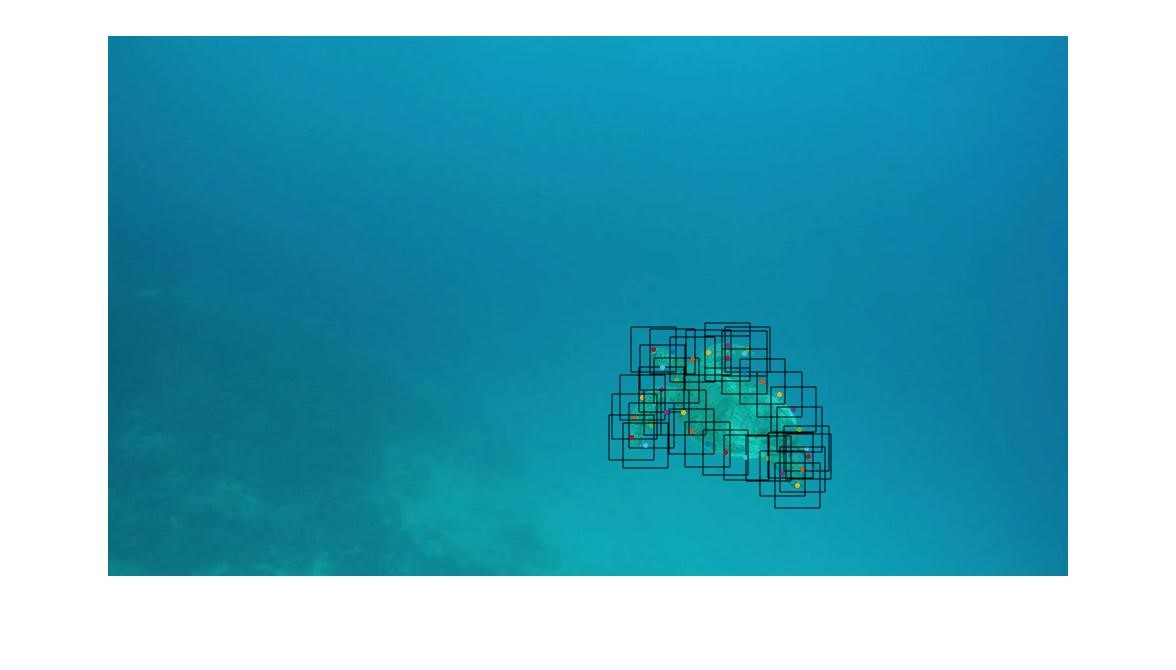
\includegraphics[width=100mm]{img/i10}
	\end{center}

	\section{Update Color Model (and color confidence)}
	For updating the color model and color confidence, it was more difficult because there was less information in the slides. We went through the paper and attempted to follow their algorithm. For the color models, we ran the initialized GMM on each local window. Then, we got the foreground probability on each pixel and chose pixels that were 75\% likely to be in the foreground (that’s the number they used in the paper). We added those new points to the points that were used in the GMM and then fit a new GMM. Then, we ran GMM again with those new points and got new foreground probabilities for the windows.
	Then, we had to decide if we wanted the new GMM or the previous GMM. To do this, we just checked how many more points we characterized as foreground points. If it was reasonably bigger, we took the new GMM and calculated new confidences. 
	
	\section{Combine Shape and Color Models}
	For combining the shape and color models, we initialized a new shape confidence with the new color model. Then, to combine the models, we looked at each window, and used the warped mask, shape confidence, and color model probability. We used the equation from the paper for this: $$p_f^k(x)=f_s(x)L^{t+1}(x)+(1-f_s(x)p_c(x))$$
	
	\section{Merge Local Windows}
	
	To merge local windows, we went through each window and used the formula from the paper:
	
	$$p_f(x)=\frac{\Sigma_kp_f^k(x)(|x-c_k|+\epsilon)^{-1}}{\Sigma_k(|x-c_k|+\epsilon)^{-1}}$$
	
	\section{Extract Final Foreground Mask}
	For extracting the final foreground mask, we checked pf from the merging and saw if it was over our threshold of 0.5. 
	
	\section{Results}
	Our results did not turn out so good. Our local windows were updating well, but our masks were not very accurate. Below is an image of the local windows about 10 frames in. You can see that the fins are a little off, but the rest of the tracking is quite close. We got similar results for the other frames as well.
	
	\begin{center}
		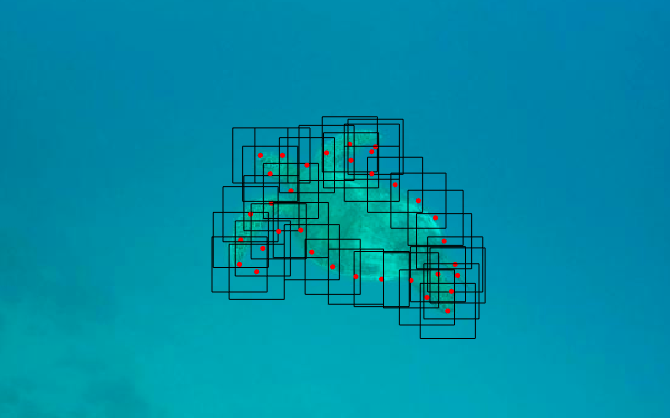
\includegraphics[width=100mm]{img/i11}
	\end{center}

	Our issues with the masks could be due to numerous things. We think that we messed up with the merging of the local models. You can see in the images below that too many points are being classified as foreground points
	Another problem that was mentioned in the paper that could’ve affected our results was luminance variance and object rotation. Most of the tracked objects had shifts in color due to light. The object in Frames 2 and 3 also rotated.
	Another issue we came across was that we couldn’t run through all the frames. An error popped up that said that we need more rows than columns for fitgmdist. We could not figure out why it was getting smaller because theoretically the points would be the same or get larger.
	Lastly, we decided to not use lazysnapping because when we tried to use it, it took a long time to compute. We couldn’t test the extraction of the mask thoroughly because our masks were not accurate, but from looking on Piazza, we figured that if our masks were accurate, they would have holes in them. To fix this hypothetical problem, we used imfill. 
	
	\subsection{Set 1 - Frames 1 through 6}
	
	\begin{center}
		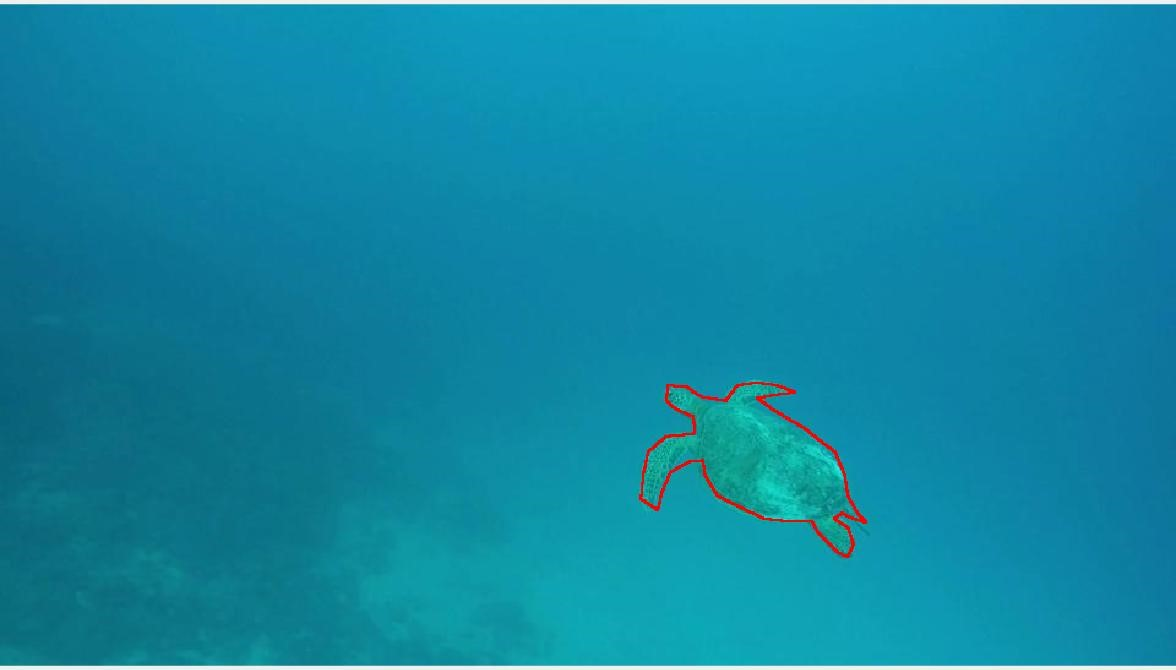
\includegraphics[width=100mm]{img/a1}
	\end{center}

	\begin{center}
		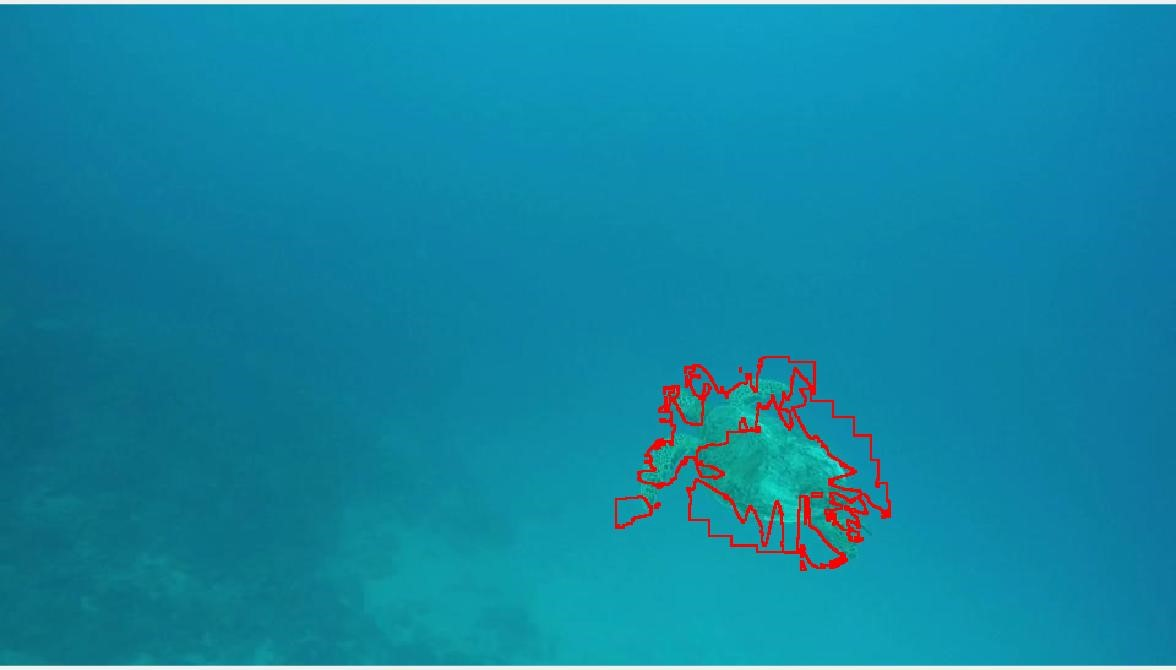
\includegraphics[width=100mm]{img/a2}
	\end{center}

	\begin{center}
		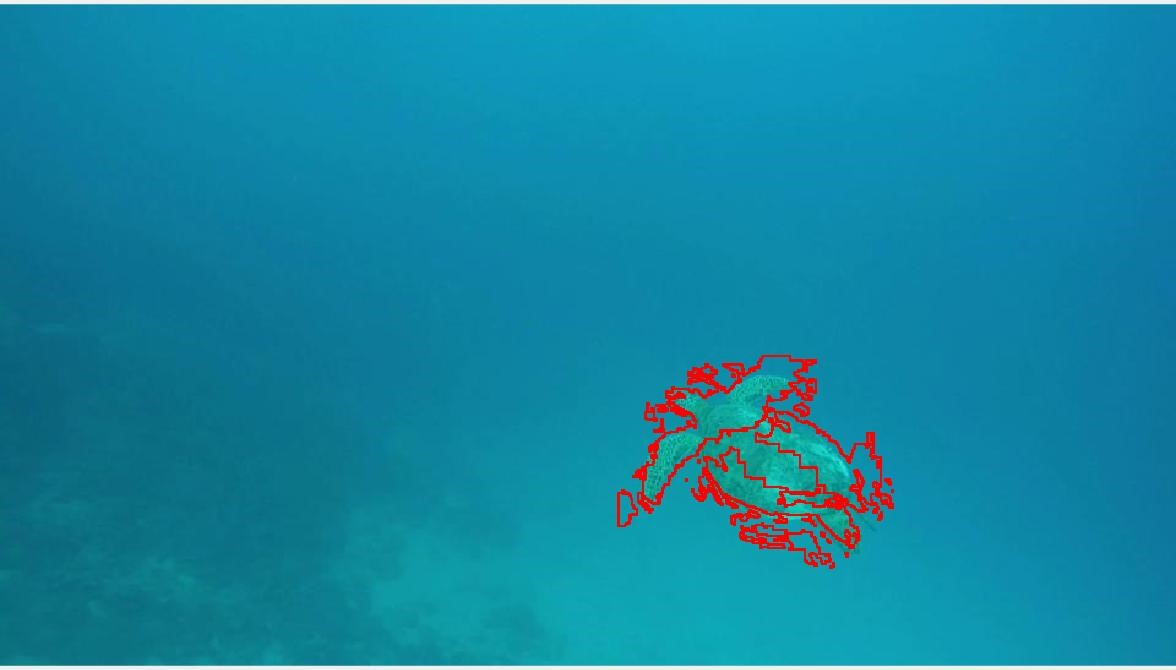
\includegraphics[width=100mm]{img/a3}
	\end{center}

	\begin{center}
		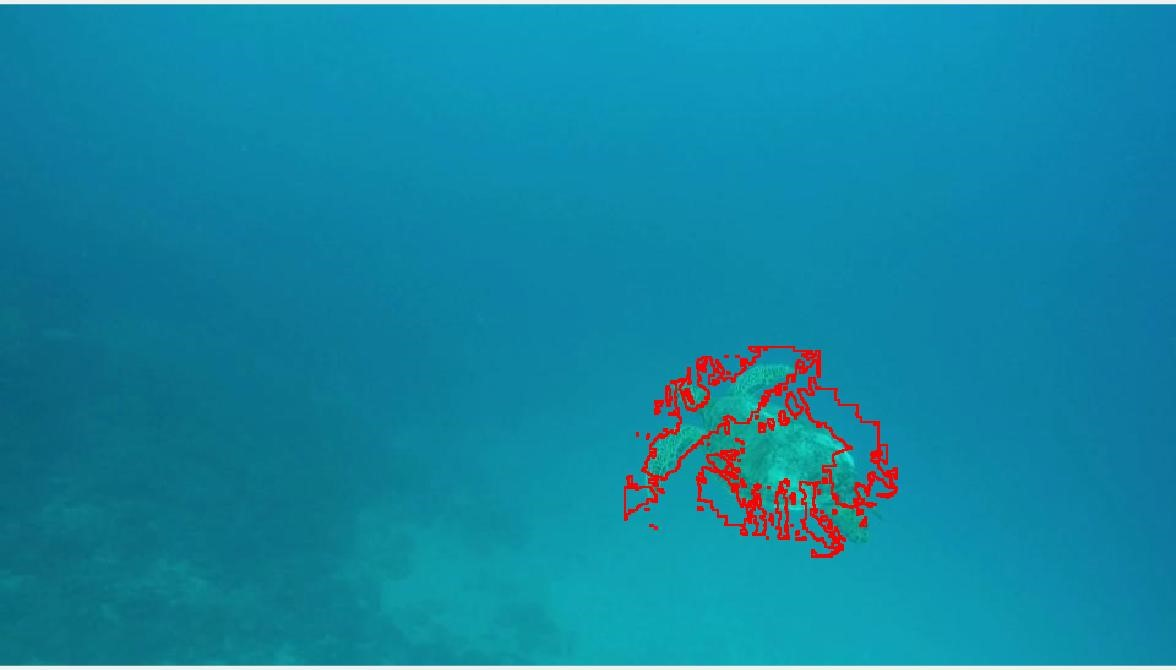
\includegraphics[width=100mm]{img/a4}
	\end{center}

	\begin{center}
		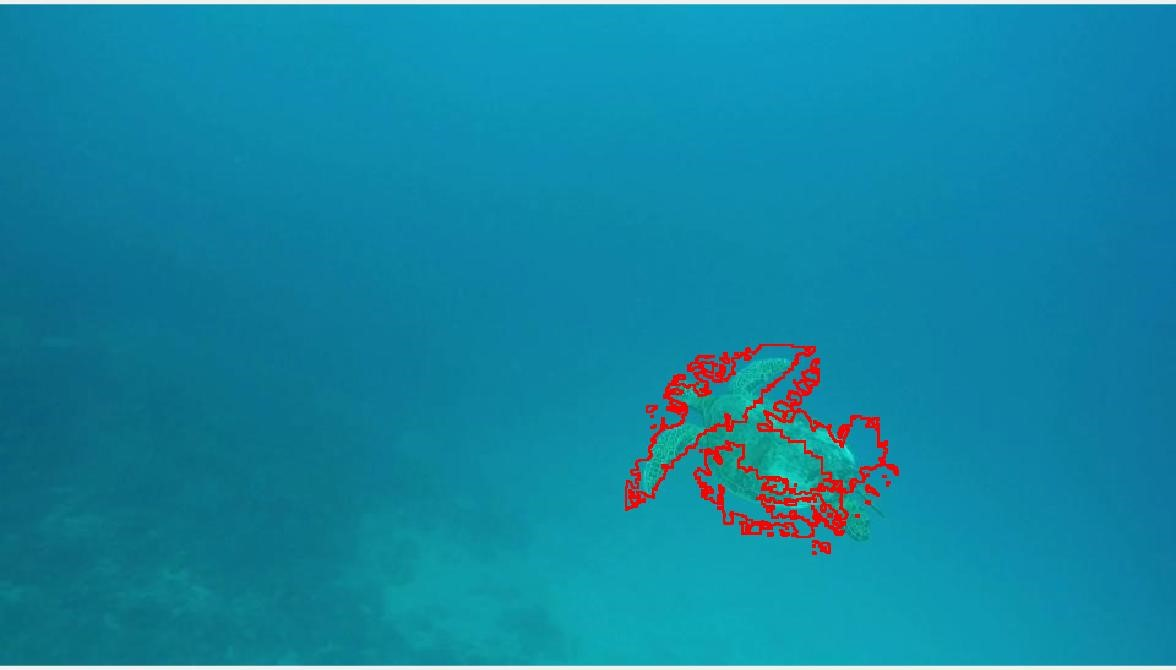
\includegraphics[width=100mm]{img/a5}
	\end{center}

	\begin{center}
		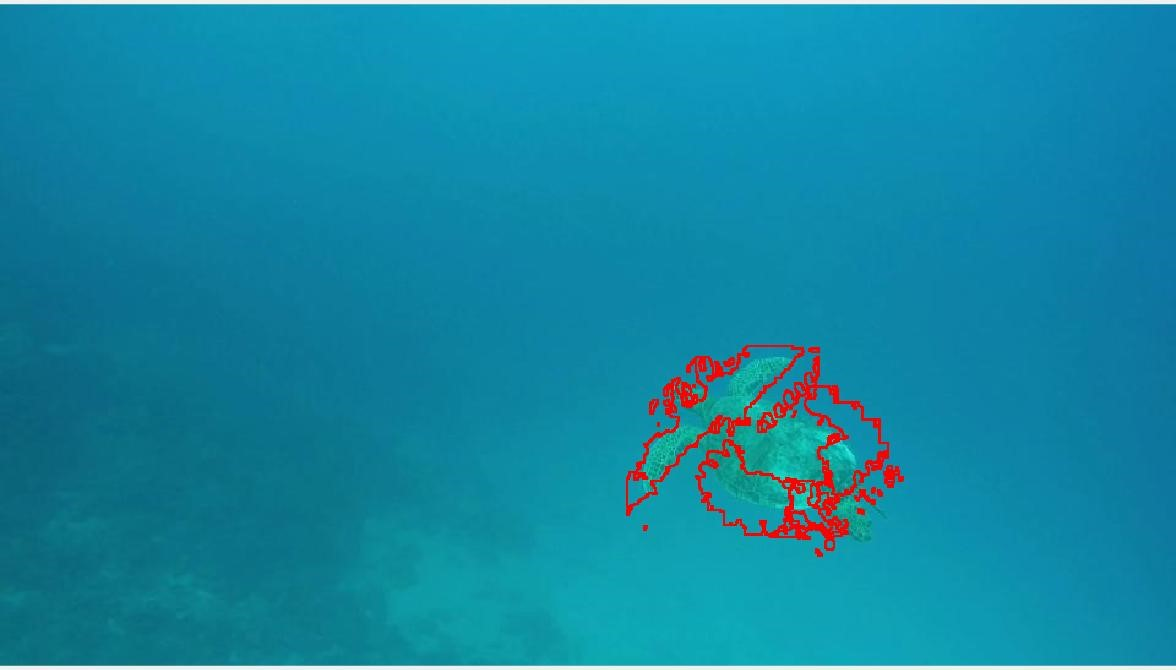
\includegraphics[width=100mm]{img/a6}
	\end{center}

	\subsection{Set 2 - Frames 1 through 6}
	
	\begin{center}
		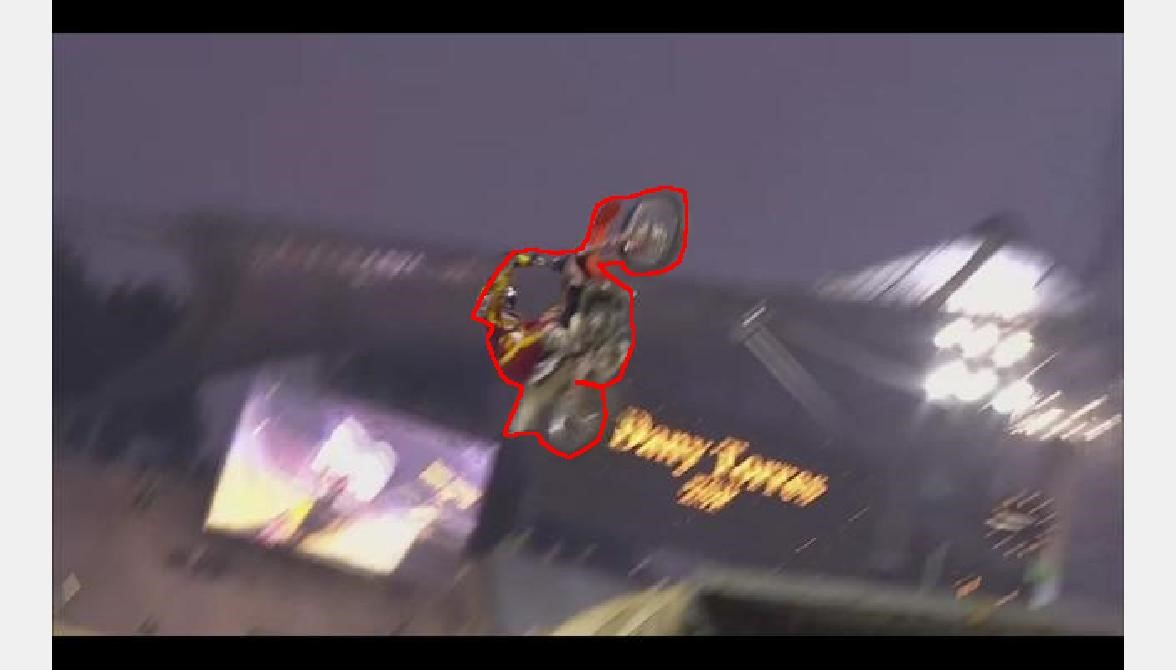
\includegraphics[width=100mm]{img/b1}
	\end{center}
	
	\begin{center}
		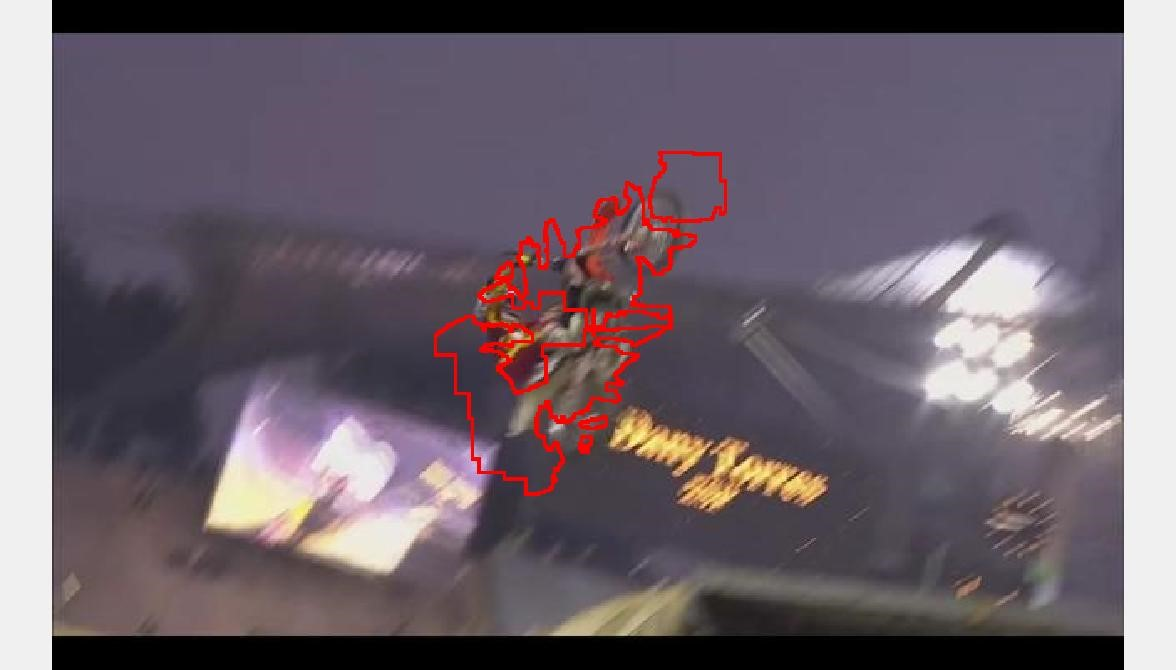
\includegraphics[width=100mm]{img/b2}
	\end{center}
	
	\begin{center}
		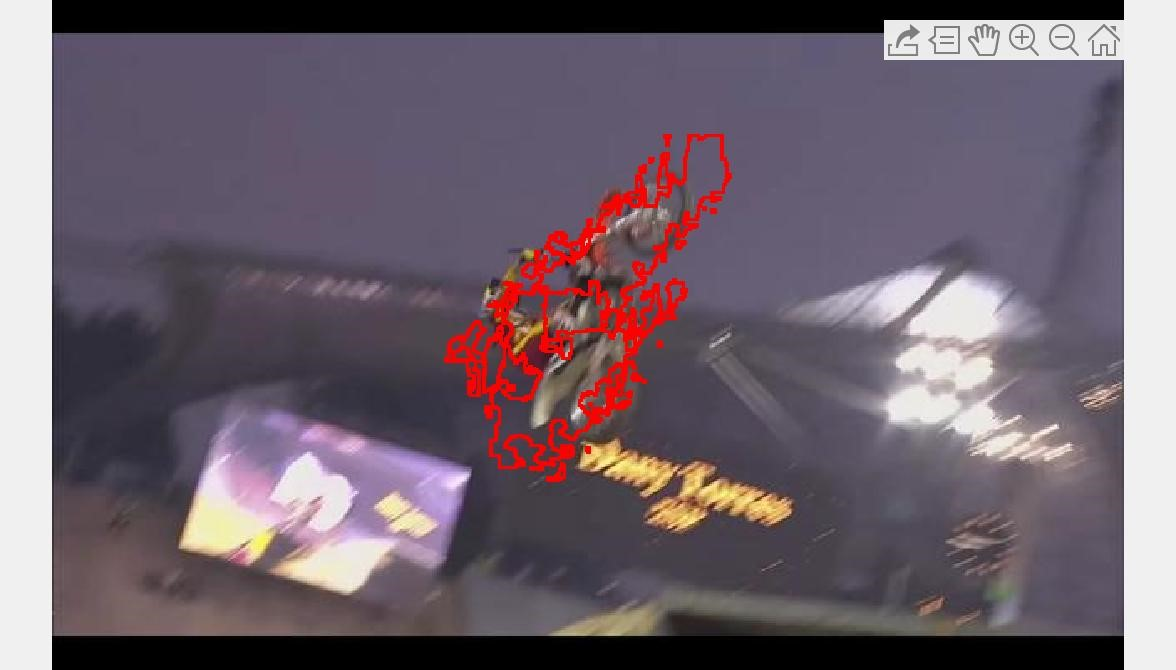
\includegraphics[width=100mm]{img/b3}
	\end{center}
	
	\begin{center}
		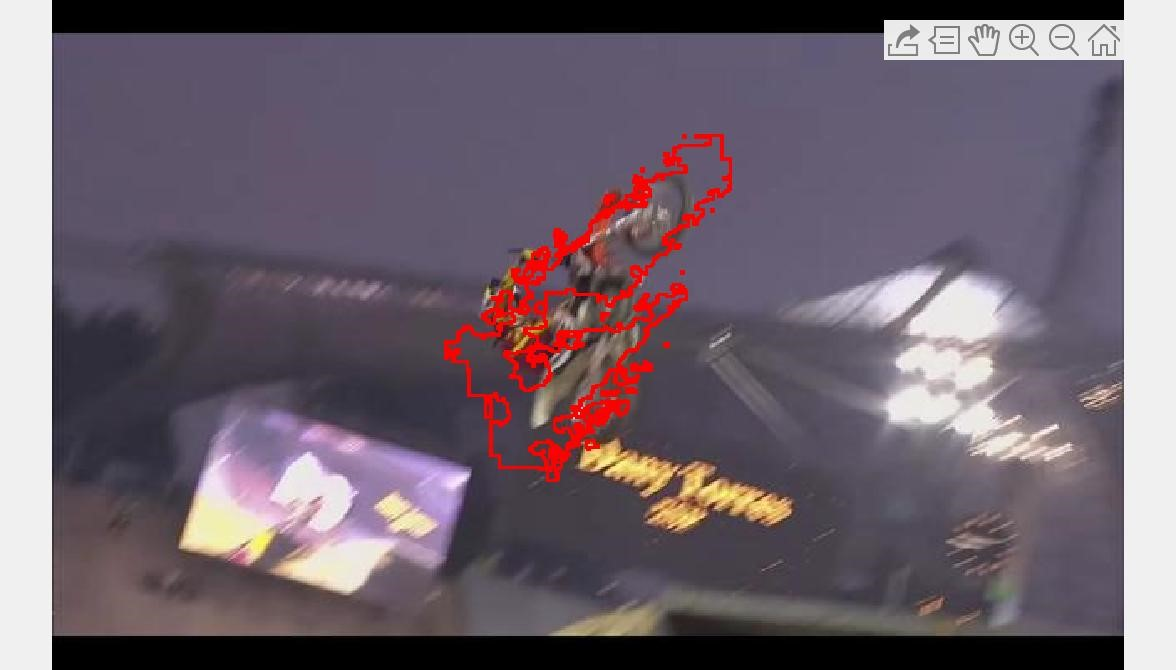
\includegraphics[width=100mm]{img/b4}
	\end{center}
	
	\begin{center}
		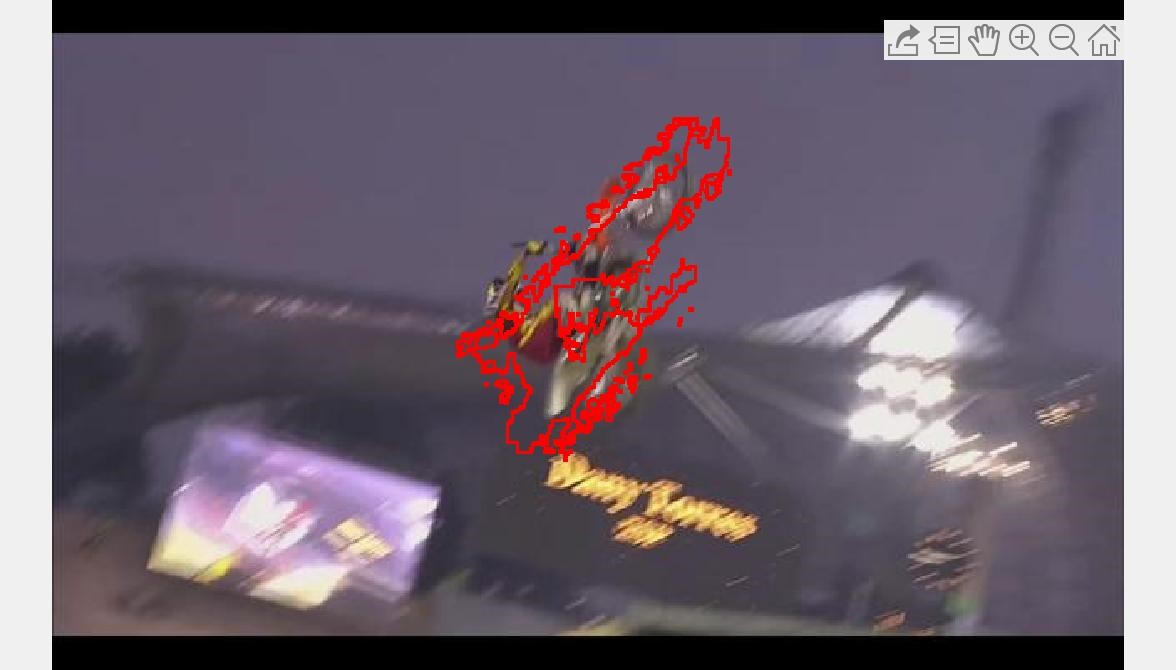
\includegraphics[width=100mm]{img/b5}
	\end{center}
	
	\begin{center}
		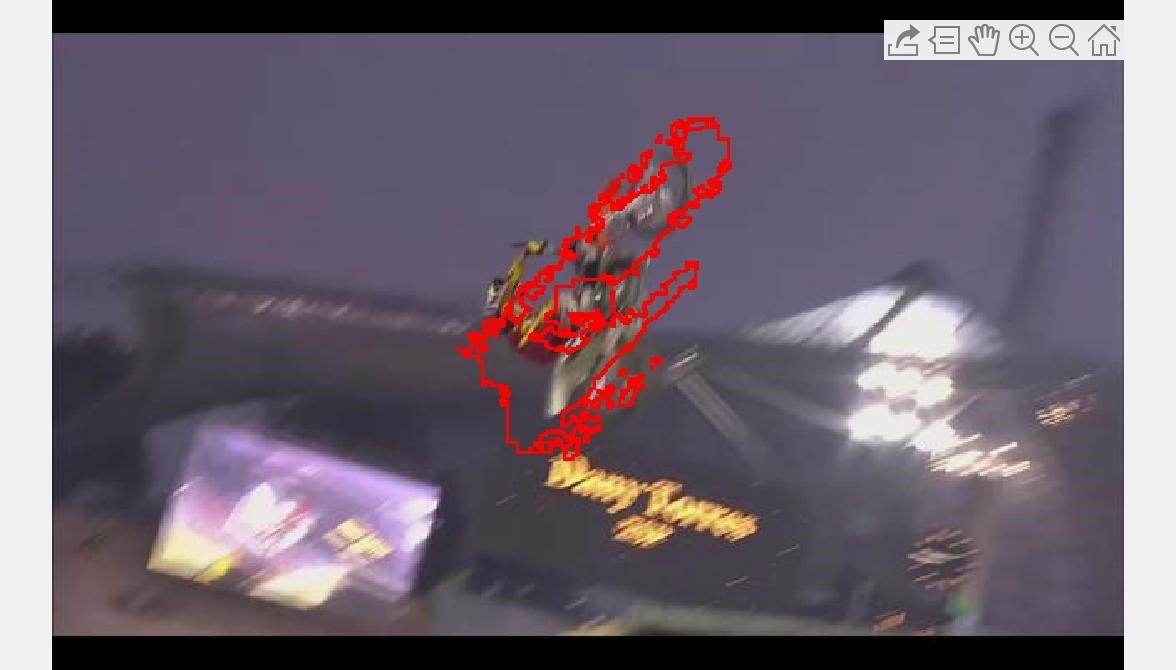
\includegraphics[width=100mm]{img/b6}
	\end{center}


	\subsection{Set 3 - Frames 1 through 6}
	
	\begin{center}
		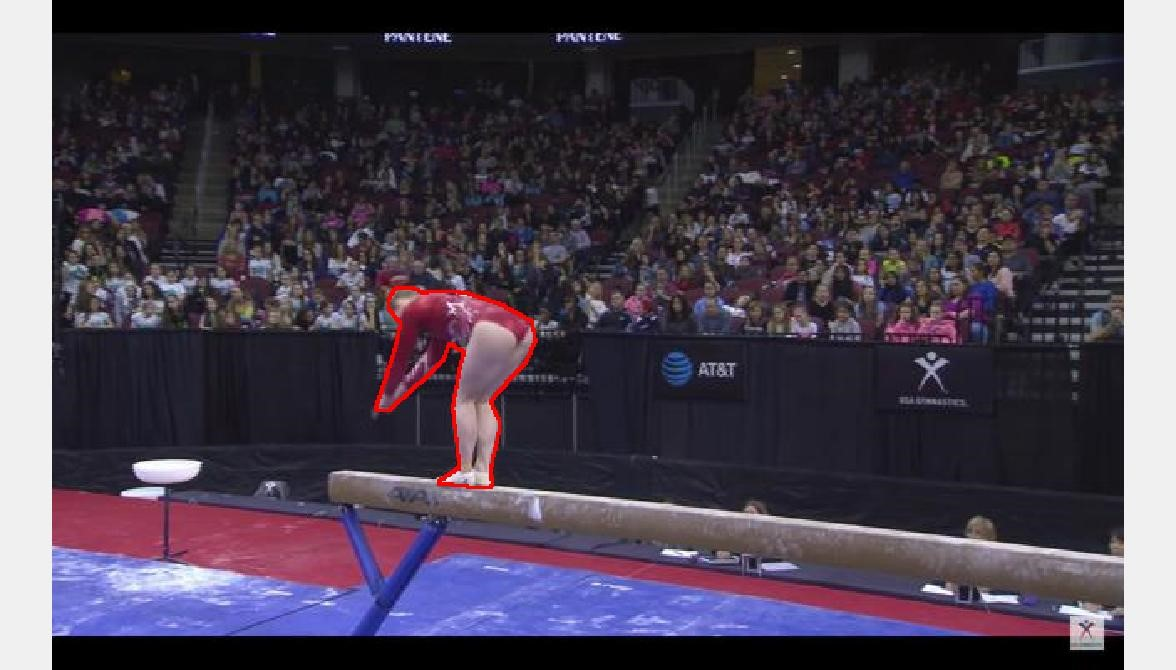
\includegraphics[width=100mm]{img/c1}
	\end{center}
	
	\begin{center}
		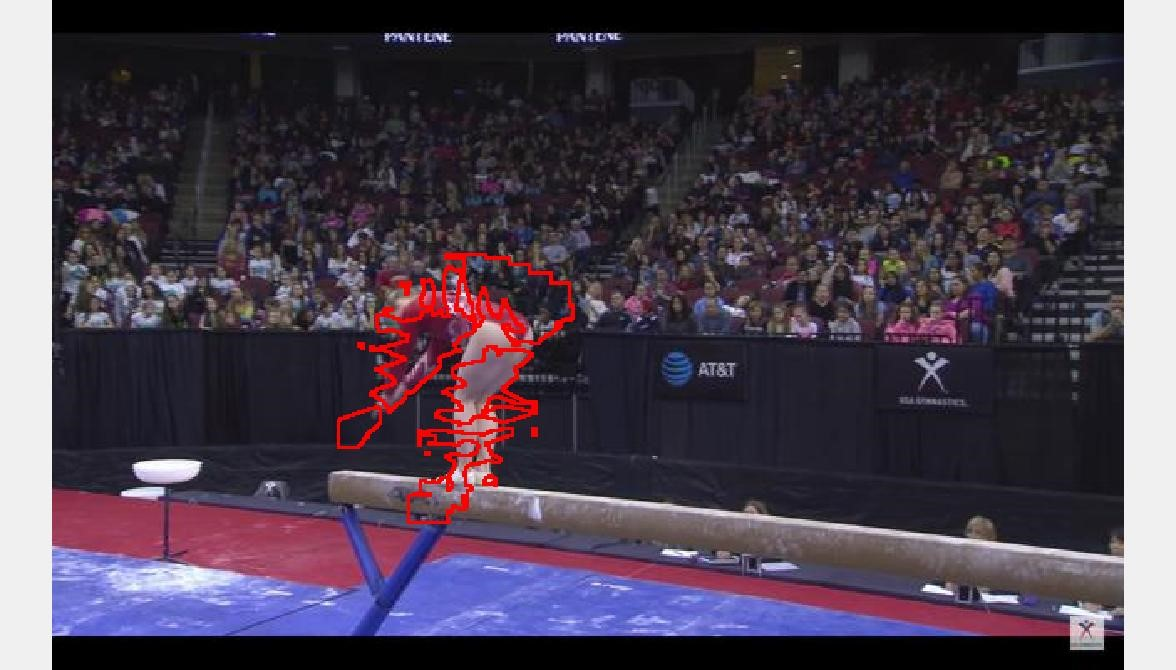
\includegraphics[width=100mm]{img/c2}
	\end{center}
	
	\begin{center}
		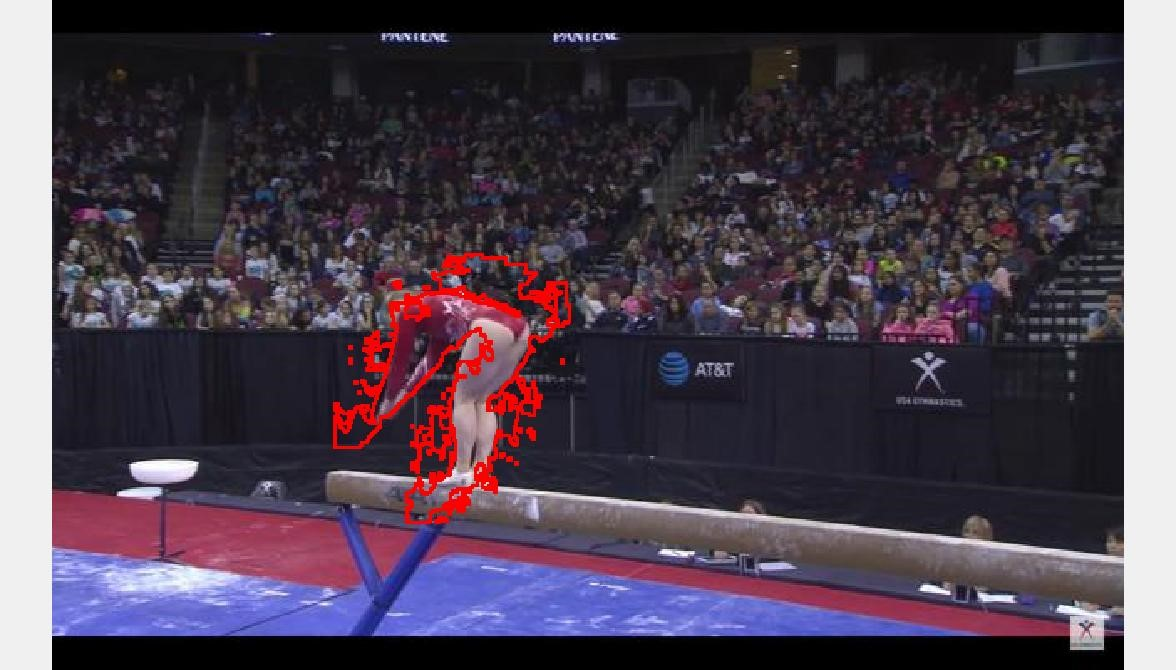
\includegraphics[width=100mm]{img/c3}
	\end{center}
	
	\begin{center}
		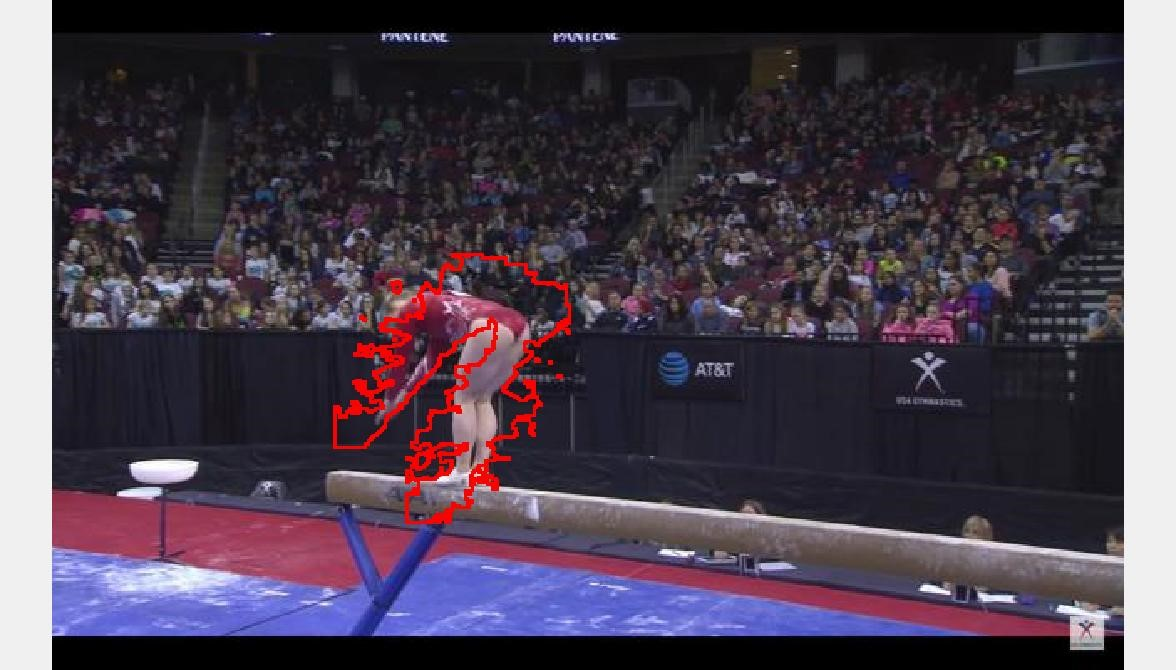
\includegraphics[width=100mm]{img/c4}
	\end{center}
	
	\begin{center}
		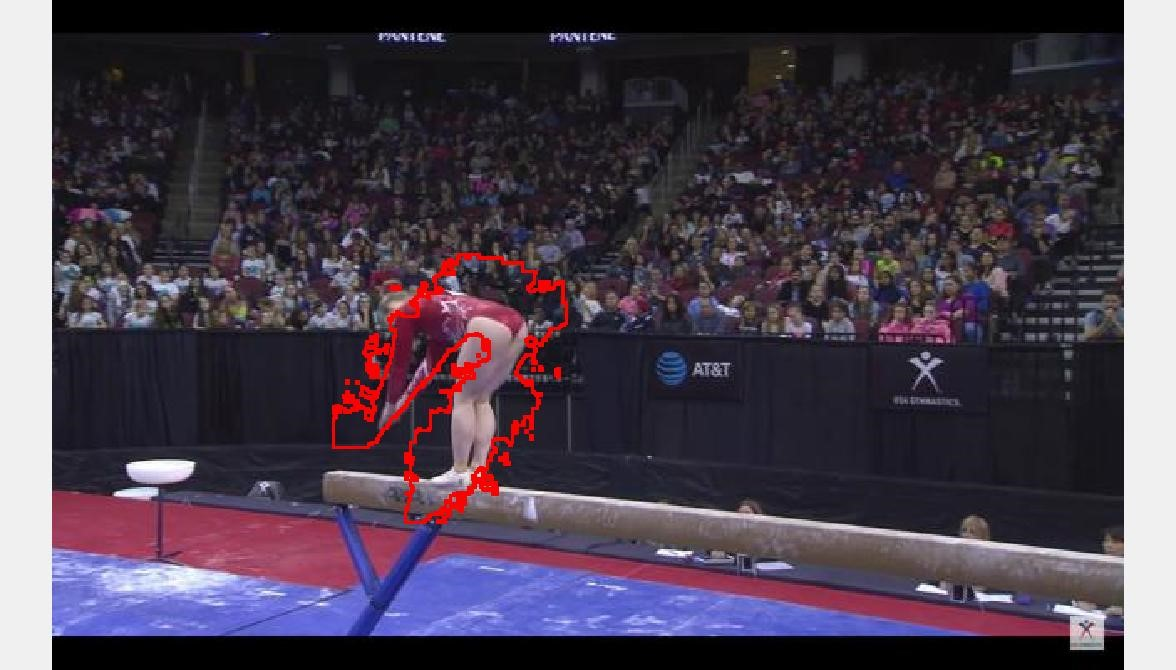
\includegraphics[width=100mm]{img/c5}
	\end{center}
	
	\begin{center}
		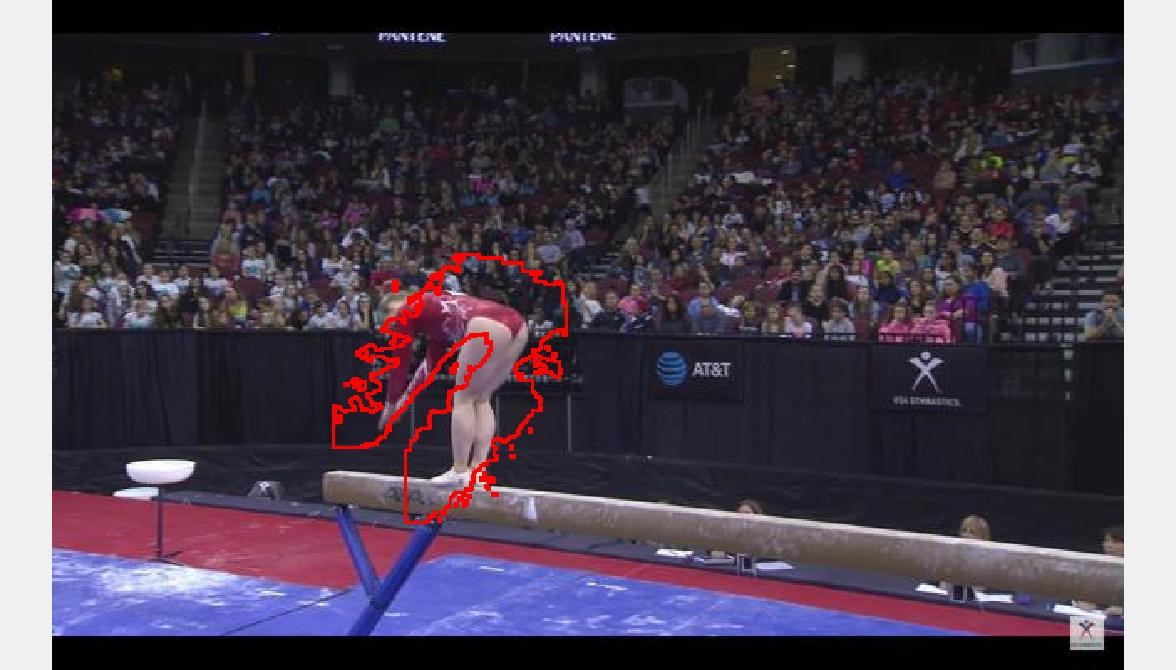
\includegraphics[width=100mm]{img/c6}
	\end{center}

	\subsection{Set 4 - Frames 1 through 6}
	
	\begin{center}
		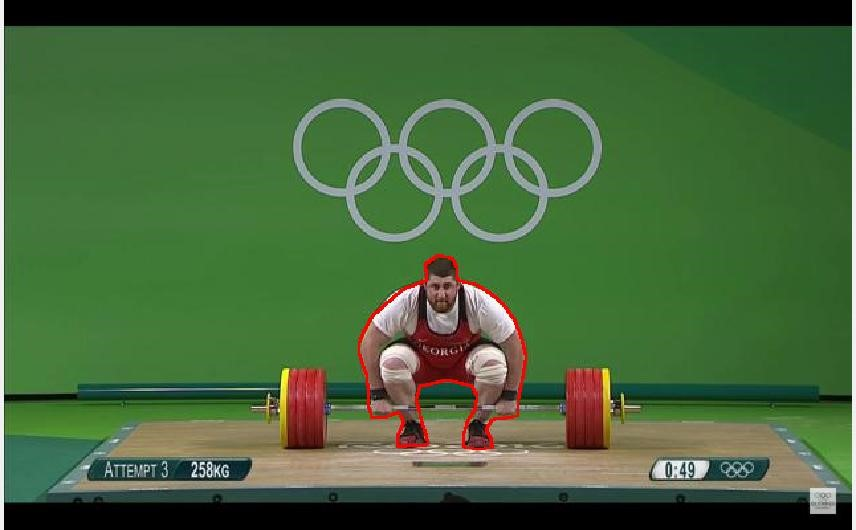
\includegraphics[width=100mm]{img/d1}
	\end{center}
	
	\begin{center}
		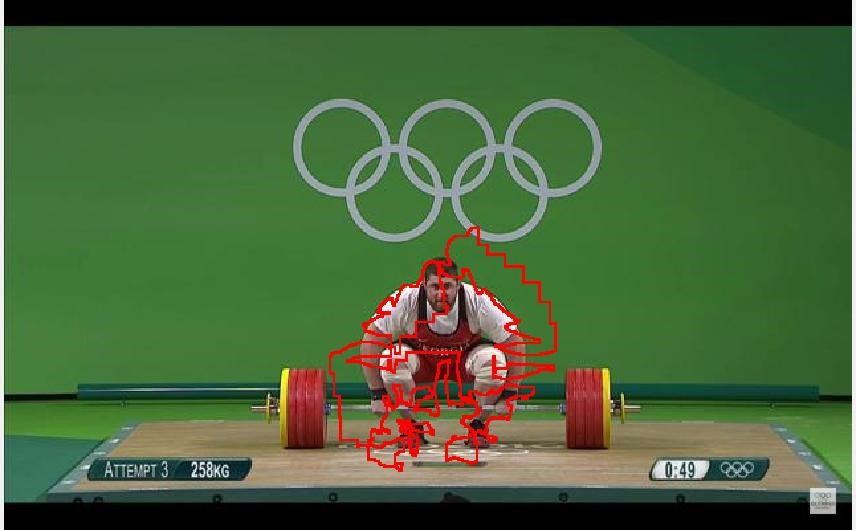
\includegraphics[width=100mm]{img/d2}
	\end{center}
	
	\begin{center}
		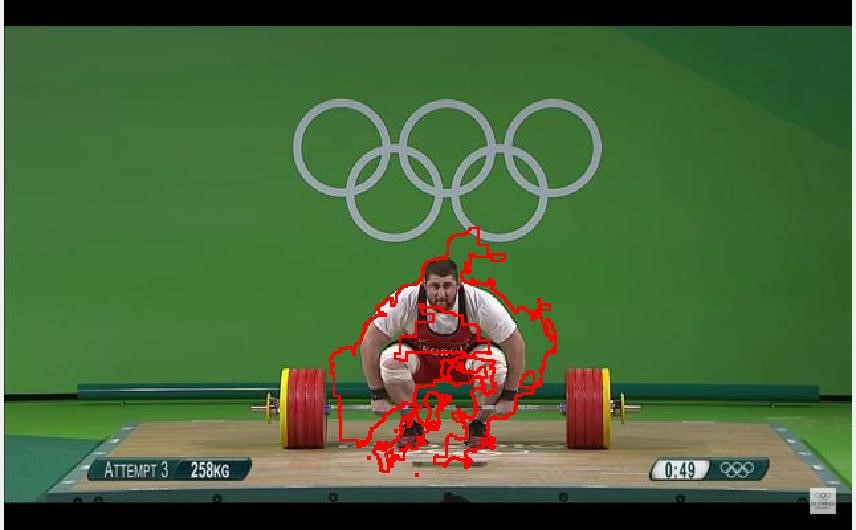
\includegraphics[width=100mm]{img/d3}
	\end{center}
	
	\begin{center}
		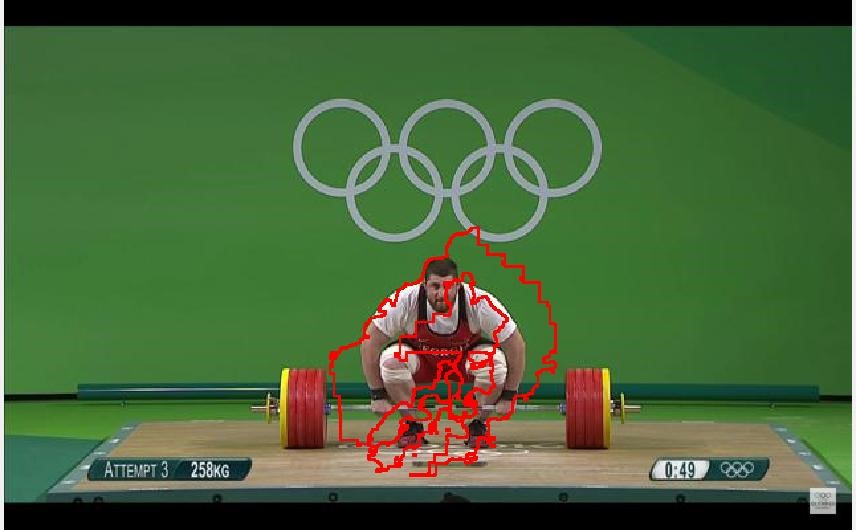
\includegraphics[width=100mm]{img/d4}
	\end{center}
	
	\begin{center}
		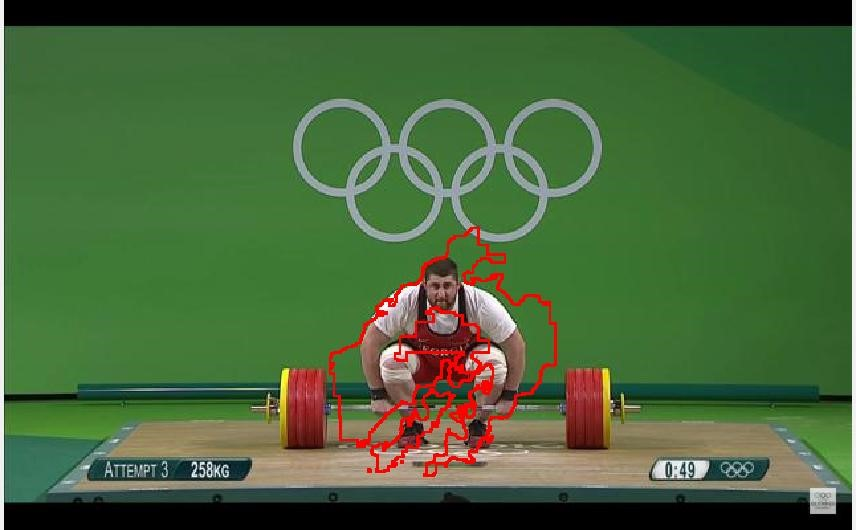
\includegraphics[width=100mm]{img/d5}
	\end{center}
	
	\begin{center}
		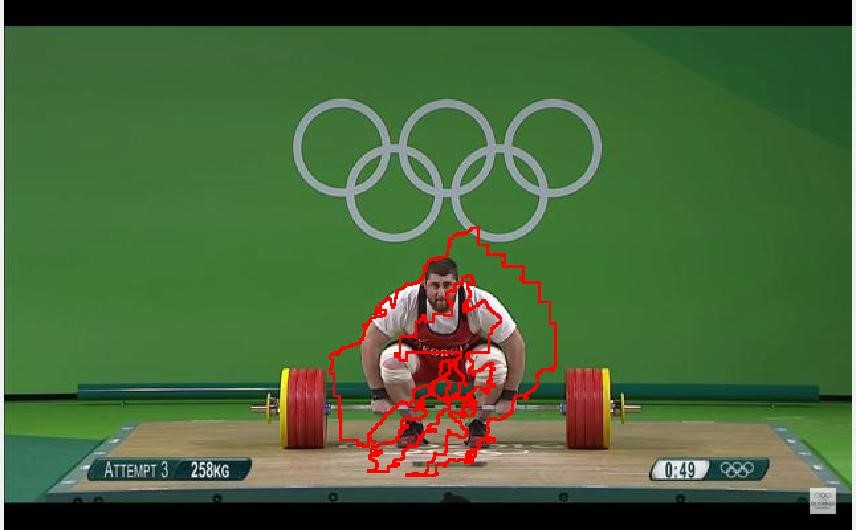
\includegraphics[width=100mm]{img/d6}
	\end{center}

	\subsection{Set 5 - Frames 1 through 6}
	
	\begin{center}
		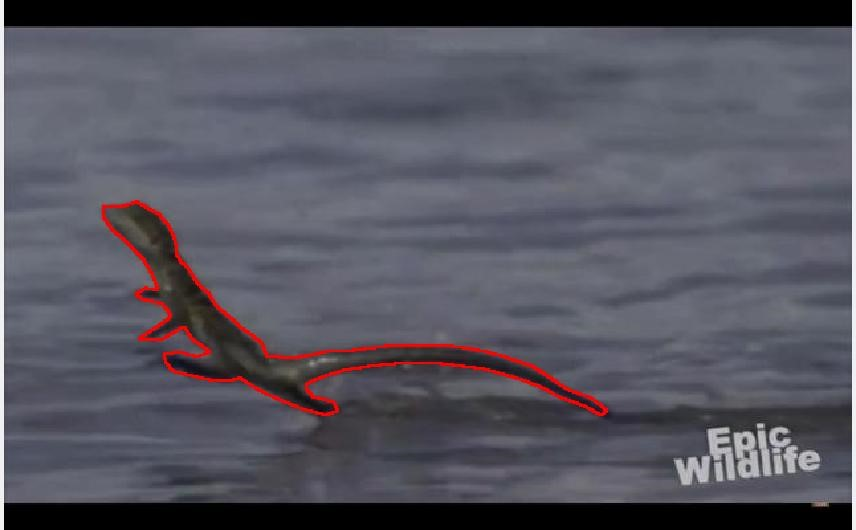
\includegraphics[width=100mm]{img/e1}
	\end{center}
	
	\begin{center}
		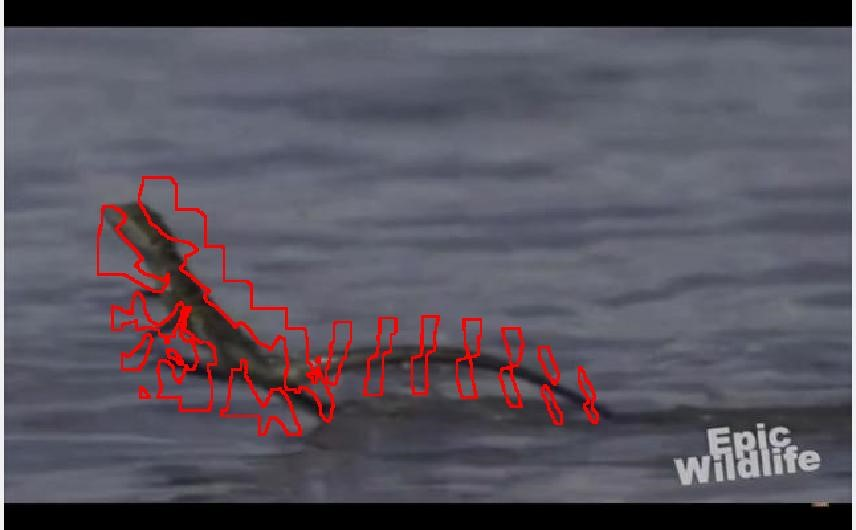
\includegraphics[width=100mm]{img/e2}
	\end{center}
	
	\begin{center}
		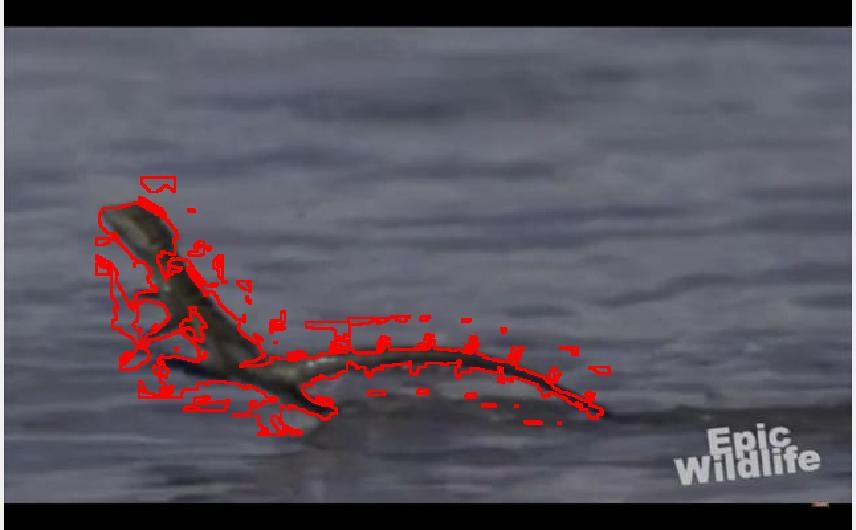
\includegraphics[width=100mm]{img/e3}
	\end{center}
	
	\begin{center}
		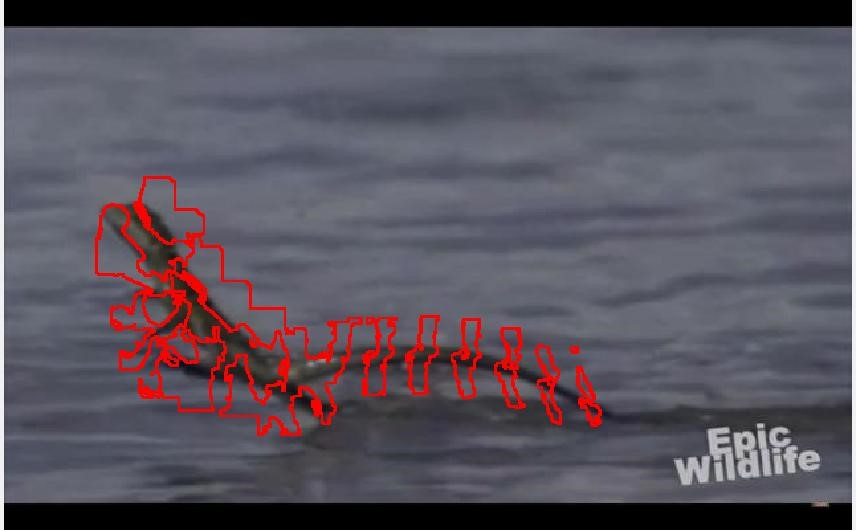
\includegraphics[width=100mm]{img/e4}
	\end{center}
	
	\begin{center}
		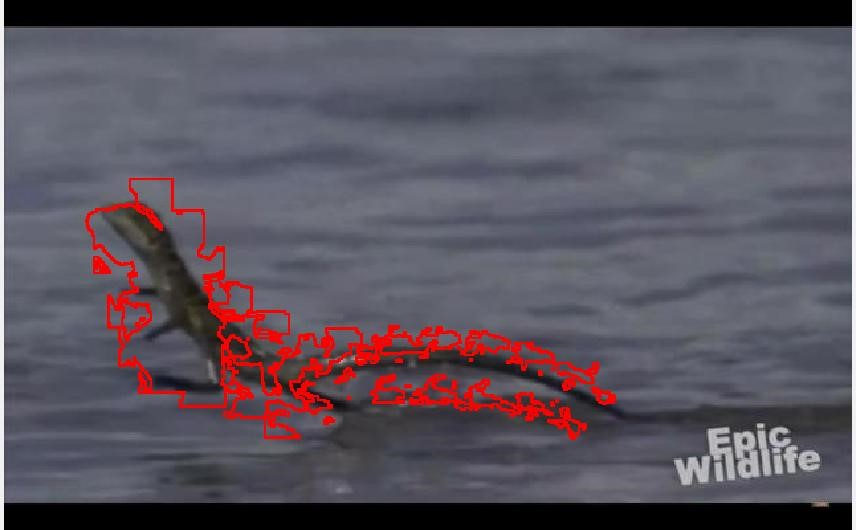
\includegraphics[width=100mm]{img/e5}
	\end{center}
	
	\begin{center}
		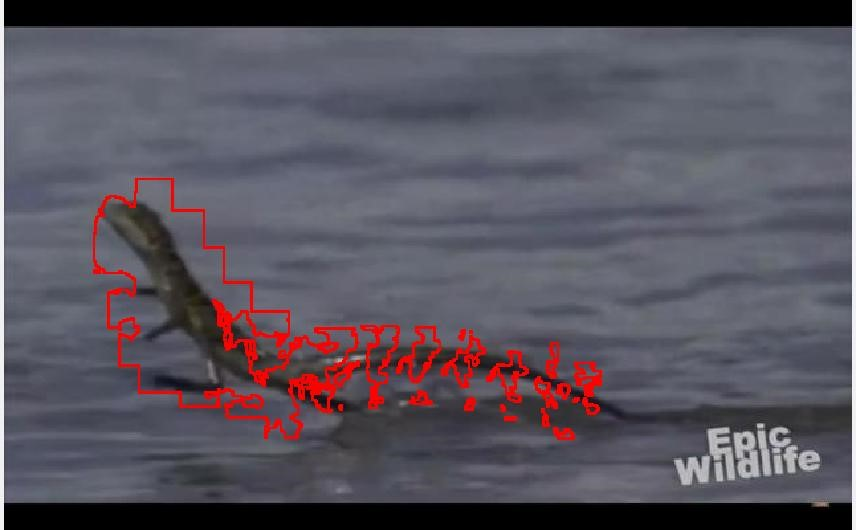
\includegraphics[width=100mm]{img/e6}
	\end{center}
	
\end{document}